
\title{Лексический анализ динамически формируемых строковых выражений}

\titlerunning{Лексический анализ динамических строковых выражений}

\author{Полубелова Марина Игоревна}

\authorrunning{М.И.Полубелова}

\tocauthor{М.И.Полубелова}
\institute{Санкт-Петербургский государственный университет\\
\email{polubelovam@gmail.com}}

\maketitle             

\begin{abstract}
test
\end{abstract}



% У введения нет номера главы
\section*{Введение}

Многие языки программирования позволяют работать со строковыми выражениями. Эти выражения могут быть получены с помощью строковых операций и языковых конструкций, например, условных операторов и циклов, то есть быть динамически формируемыми. Такие строковые выражения можно использовать, например, при генерации нового кода или при формировании запросов к базе данных. В качестве примера использования динамически формируемого строкового выражения рассмотрим SQL-запрос в C\#:    

\fvset{frame=lines,framesep=5pt}
\begin{listing}[H]
    \begin{lstlisting}[language=csharp]
 private void Go(bool cond)
 {
   string tableName = cond ? "Sold" : "OnSale ";
   string queryString =
       "SELECT ProductID, UnitPrice, ProductName " 
           + "FROM dbo.products_" + tableName
           + "WHERE UnitPrice > 1000 "
           + "ORDER BY UnitPrice DESC;";
   Program.ExecuteImmediate(queryString);
 }
    \end{lstlisting}
\caption{Пример встроенного SQL в C\#}
\label{lst:verbments}
\end{listing}

В этом примере выполняется запрос к базе данных (строка 9), в котором сам запрос получен в результате конкатенации нескольких строк (строки 5 -- 8), выполненной с помощью условного оператора (строка 3). В строке 3 при формировании имени таблицы пропущен пробел, что приведет к ошибке выполнения запроса в случае истинности выражения \verb|cond|. Но об ошибках подобного рода мы узнаем только в момент выполнения программы. На этом же примере видно, что в строке выполнения запроса (строка 9) содержится множество значений динамически формируемого строкового выражения \verb|queryString|, компактное представление которого также хотелось бы иметь при разработке таких программ.

Динамически формируемые строковые выражения воспринимаются компилятором как обычные строки, что делает систему, использующую такой подход, ненадежной и уязвимой. Несмотря на то, что сейчас распространены другие технологии разработки программ, использующих язык запросов SQL, например LINQ, обозначенная выше проблема все равно остается актуальной. Во-первых, существует множество  уже написанных программ и систем с использованием динамически формируемых строковых выражений, которые необходимо поддерживать. Во-вторых, может потребоваться реинжиниринг этих программ. Например, если выполнять миграцию системы с языка Transact-SQL на Oracle-SQL, то тогда в приведенном выше примере необходимо формировать запрос уже на другом языке и при этом необходимо сохранить связь преобразованного кода с исходным. Так как в результате миграции  могут возникнуть новые имена переменных, функций и другие языковые конструкции, то пользователям системы нужно быть уверенным в том, что логика и объекты системы не изменились. В-третьих, в web-программировании широко используется такой подход, например, динамически генерируемый HTML в PHP-программах. То есть в этом случае необходим статический анализ динамически формируемых строковых выражений.    

Таким образом, ставится вопрос корректности программ, получающихся в результате использования динамически формируемых строковых выражений. Один из подходов к анализу таких программ заключается в проверке включения языков~\cite{JSA1, PHPSA}. Этот подход только отвечает на вопрос, включается ли язык, который порождает программа, в язык, описанный пользователем. Следующий подход состоит в проведении лексического анализа и синтаксического разбора компактного представления множества динамически формируемых строковых выражений, в качестве которого может быть регулярное выражение~\cite{Alvor1} или data-flow уравнение~\cite{Doh}. Этот подход позволяет для динамически формируемых строковых выражений разработать такую же функциональность, которую предоставляют интегрированные среды разработки для обычных языков, например, автодополнение, рефакторинг и дополнительные статические проверки.

Существуют инструменты, которые реализуют рассмотренные подходы, например, Java String Analyzer \cite{JSA1}, PHP String Analyzer \cite{PHPSA} и Alvor \cite{Alvor1}. Однако они обладают рядом недостатков, среди которых можно выделить низкую точность проводимого анализа и трудность добавления поддержки нового языка. Последний недостаток можно заменить автоматизированным процессом, использовав, например, стандартные генераторы лексических и синтаксических анализаторов. В статье~\cite{LexerAdv} были показаны преимущества проведения лексического анализа отдельно от синтаксического разбора. Одним из преимуществ лексического анализа является то, что он не вносит потери точности проводимого анализа, а также позволяет переиспользовать существующие определения грамматик. В данной работе, выполненной в рамках проекта YaccConstructor~\cite{YC_article}, будет представлена реализация инструмента для проведения лексического анализа выражений, которые могут быть получены с помощью строковых операций и циклов, с сохранением привязки к исходному коду. В этой работе также будет представлена реализация генератора лексических анализаторов, что позволит сравнительно легко добавить обработку нового языка в реализованный инструмент.


\section{Постановка задачи}
Целью данной работы является реализация инструмента для проведения лексического анализа динамически формируемых строковых выражений. Для её достижения были поставлены следующие задачи:

\begin{itemize}
\item реализовать механизм для лексического анализа выражений, формируемых с помощью циклов и строковых операций, сохраняющий привязку частей динамически формируемого строкового выражения к исходному коду и привязку лексических единиц внутри каждой части;
\item реализовать генератор лексических анализаторов, который по заданной спецификации языка строит описание конечного преобразователя. Конечный преобразователь --- это конечный автомат, который может выводить конечное число символов для каждого входного символа.
\end{itemize}


\section{Обзор}

\subsection{Конечные преобразователи}

\textbf{Конечный преобразователь} (Finite State Transducer,~\cite{FST}) {---} это конечный автомат~(Finite State Automata,~\cite{FSA}), который может выводить конечное число символов для каждого входного символа. Конечный преобразователь может быть задан следующей шестеркой элементов: $\langle Q, \Sigma, \Delta, q_0, F, E \rangle$, где

\begin{itemize}
\item $Q$ --- множество состояний, 
\item $\Sigma$ --- входной алфавит, 
\item $\Delta$ --- выходной алфавит, 
\item $q_0 \in Q$ --- начальное состояние, 
\item $F \subseteq Q$ --- набор конечных состояний, 
\item $E \subseteq Q \times (\Sigma \cup \{\varepsilon\}) \times (\Delta \cup \{\varepsilon\})  \times Q$ --- набор переходов. 
\end{itemize}

Конечные преобразователи находят широкое применение в области обработки естественного языка (Natural Language Processing, \cite{Mohri}), также их можно использовать и при проведении лексического анализа. Важной операцией над конечными преобразователями является операция композиция. \textbf{Композиция} конечных преобразователей~{---}~это два стоящих рядом  взаимодействующих конечных преобразователя, работающих таким образом: выход первого конечного преобразователя является входом для второго конечного преобразователя. Ниже дано формальное определение операции композиция над конечными преобразователями, допускающие наличие \verb|eps|-переходов.

\textbf{Композицией} двух конечных преобразователей $T_1~=~\langle Q_1, \Sigma_1, \Delta_1, q_{0_{1}}, F_1, E_1 \rangle$ и $T_2~=~\langle Q_2, \Sigma_2, \Delta_2, q_{0_{2}}, F_2, E_2 \rangle$ является конечный преобразователь  $T =\langle Q_1  \times Q_2, \Sigma_1, \Delta_2, \\ \langle q_{0_{1}}, q_{0_{2}} \rangle, F_1 \times F_2, E \cup E_{\varepsilon} \cup E_{i,\varepsilon} \cup E_{o,\varepsilon} \rangle$, где 

\begin{itemize}
\item $E = \{ \langle \langle p, q \rangle, a, b, \langle p', q' \rangle \rangle\ | \exists c \in \Delta_1 \cap \Sigma_2 : \langle p, a, c, p' \rangle \in E_1 \wedge \langle q, c, b, q' \rangle \in E_2\}$
\item $E_{\varepsilon} = \{ \langle \langle p, q \rangle, a, b, \langle p', q' \rangle \rangle\ | \langle p, a, {\varepsilon}, p' \rangle \in E_1 \wedge \langle q, {\varepsilon}, b, q' \rangle \in E_2\}$
\item $E_{i, \varepsilon} = \{ \langle \langle p, q \rangle, {\varepsilon}, a, \langle p, q' \rangle \rangle\ | \langle q, {\varepsilon}, a, q' \rangle \in E_2 \wedge p \in Q_1 \} $
\item $E_{o, \varepsilon} = \{ \langle \langle p, q \rangle,  a, {\varepsilon}, \langle p', q \rangle \rangle\ | \langle p, a, {\varepsilon}, p' \rangle \in E_1 \wedge q \in Q_2 \}. $
\end{itemize}


\subsection{Обзор существующих инструментов}

Для работы с динамически формируемыми строковыми выражениями существует ряд инструментов, которые реализуют два основных подхода. Первый подход заключается в проверке включения языков. Данный подход только отвечает на вопрос, включается ли язык, который порождает программа, в язык, описанный пользователем, например, с помощью грамматики или простым перечислением строковых выражений, которых он ожидает получить в результате выполнения программы. Его реализуют инструменты, представленные ниже.

\begin{itemize}
\item \textbf{Java String Analyzer} (JSA, \cite{JSA1, JSAUrl}) {---}  инструмент для анализа формирования строк и строковых операций в программах на Java. Для каждого строкового выражения строится конечный автомат, представляющий приближенное значение всех значений этого выражения, которые могут быть получены во время выполнения программы. Для того, чтобы получить этот конечный автомат, необходимо из flow-графа анализируемой программы построить контекстно-свободную грамматику, которая получается в результате замены каждой строковой переменной нетерминалом, а каждой строковой операции {---} правилом продукции. После чего полученная грамматика аппроксимируется регулярным языком. В качестве результата работы данный инструмент также выдает строки, которые не входят в описанный пользователем язык, но могут сформироваться во время исполнения программы. 

\item \textbf{PHP String Analyzer} (PHPSA, \cite{PHPSA, PHPSAUrl}) {---} инструмент для статического анализа строк в программах на PHP. Расширяет подход предыдущего инструмента JSA. Отсутствует этап преобразования контекстно-свободной грамматики в регулярный язык, что повышает точность проводимого анализа. Для обработки строковых операций используется конечный преобразователь, который позволяет оставаться в рамках контекстно-свободной грамматики. Дальнейший анализ строковых выражений полностью взят из инструмента JSA.
\end{itemize} 

Второй подход заключается в проведении лексического анализа и синтаксического разбора компактного представления множества динамически формируемых выражений. Данный подход реализуют инструменты, представленные ниже.

\begin{itemize}    
\item \textbf{Alvor}~\cite{Alvor, AlvorUrl} {---} плагин к среде разработки Eclipse, предназначенный для статической валидации SQL-выражений, встроенных в Java. Для компактного представления множества динамически формируемого строкового выражения используется понятие абстрактной строки, которая фактически является регулярным выражением над используемыми в строке символами. В инструменте Alvor отдельным этапом выделен лексический анализ. Поскольку абстрактную строку можно преобразовать в конечный автомат, то лексический анализ заключается в преобразовании этого конечного автомата в конечный автомат над токенами при  использовании конечного преобразователя, полученного генератором JFlex. Несмотря на то, что абстрактная строка позволяет конструировать строковые выражения при участии циклов, плагин сообщает о том, что не может поддержать такие языковые конструкции~(см.рис.~\ref{fig:alvor2}). Также инструмент Alvor не поддерживает обработку строковых операций, за исключением конкатенации~(см. рис.~\ref{fig:alvor3}).

%\begin{figure}[h!]
%\begin{center}
%\includegraphics[width=0.6\textwidth]{alvor1}
%\caption{Формирование строкового выражения с помощью цикла while в среде разработке Eclipse с установленным плагином Alvor}
%\label{fig:alvor1} 
%\end{center}
%\end{figure}

\begin{figure}[h!]
\begin{center}
\begin{tabular}{  c  c }
\begin{minipage}{\textwidth}
  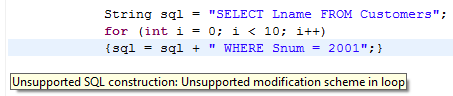
\includegraphics[width=\linewidth]{Polubelova/alvor2.png}
\end{minipage}\\    
\begin{minipage}{\textwidth}
  \includegraphics[width=\linewidth]{Polubelova/alvor1.png}
\end{minipage}
\end{tabular}    
\caption{Формирование строкового выражения с помощью цикла for и while в среде разработке Eclipse с установленным плагином Alvor}
\label{fig:alvor2} 
\end{center}
\end{figure}

\begin{figure}[h!]
\begin{center}
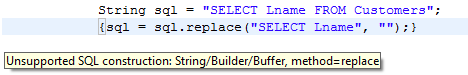
\includegraphics[width=\textwidth]{Polubelova/alvor3.png}
\caption{Формирование строкового выражения с помощью строковой операции replace  в среде разработке Eclipse с установленным плагином Alvor}
\label{fig:alvor3} 
\end{center}
\end{figure}


\item \textbf{Абстрактный синтаксический анализ}. Kyung-Goo Doh,  Hyunha Kim, David A. Schmidt в статье~\cite{Doh} описали алгоритм статического анализа динамически формируемых строковых выражений на примере статической валидации динамически генерируемого HTML в PHP-программах. Хотя для данного примера отсутствует этап проведения лексического анализа, в общем случае можно использовать композицию лексического анализа и синтаксического разбора. Для этого достаточно хранить состояние конечного преобразователя, который используется для лексического анализа, внутри состояния синтаксического разбора. Данный алгоритм также предусматривает обработку строковой операции \verb|string-replacement| с использованием конечного преобразователя, который по аналогии с лексическим конечным преобразователем хранит свое состояние внутри состояния синтаксического разбора. На вход абстрактный парсер принимает data-flow  уравнения, составленные из исходного кода, и  LALR(1) - таблицу, в качестве результата выдает набор абстрактных синтаксических деревьев.
\end{itemize}

Данный обзор показывает необходимость в реализации инструмента для проведения анализа строковых выражений, формируемых с помощью циклов и строковых операций, с сохранением привязки частей динамически формируемого строкового выражения к исходному коду и привязки лексических единиц внутри каждой части. Данная привязка может использоваться, например, при формировании сообщений об ошибках пользователю, а также при проведении реинжиниринга, для которого важно сохранить связь с исходным кодом. Для обработки языка, используемого в динамически формируемом строковом выражении, необходимо также реализовать генератор лексических анализаторов, который по спецификации обрабатываемого языка строит описание конечного преобразователя. В данной работе будет представлена реализация инструмента для проведения лексического анализа динамически формируемых строковых выражений. Преимущества проведения лексического анализа отдельно от синтаксического разбора следующие ~\cite{LexerAdv}: во-первых, при таком подходе проще обнаружить причину ложного срабатывания проводимого анализа; во-вторых, лексический анализ не вносит потери точности анализа; в-третьих, можно переиспользовать существующие определения грамматик языков.

\subsection{Средства обработки строковых операций}

Поскольку динамически формируемые строковые выражения могут быть получены и при участии строковых операций, то их обработку также стоит включить в проводимый анализ. При этом некоторые из этих операций могут быть выражены через строковую операцию \verb|replace|. Для реализации обработки этой операции, каждый аргумент которой является конечным автоматом, использовался алгоритм, описанный в статье~\cite{ReplaceFangYu}. Данный алгоритм реализован в инструменте Stranger~\cite{StrangerFangYu}, который предназначен для верификации строковых операций в PHP программах. В этом инструменте динамически формируемые строковые выражения представлены посредством конечного автомата с использованием библиотеки MONA~\cite{MONAUrl}, которая написана на языке программирования C и для конечного автомата использует MBDD-представление~\cite{MBDD}. По причине того, что для символов алфавита конечного автомата необходимо хранить дополнительную информацию, инструмент Stranger не используется в данной работе.

Инструмент Stranger подразумевает только получение строк, которые могут быть получены в результате выполнения программы и при этом являться причиной уязвимости этой программы. Для достижения этой цели необходимо выполнить операцию пересечения конечного автомата, представляющий приближенное значение всех значений обрабатываемого выражения, которые могут быть получены во время выполнения, с конечным автоматом, который является шаблоном для поиска уязвимости в программах. То есть реализация инструмента Stranger не подразумевает проведение лексического анализа и синтаксического разбора множества динамически формируемых строковых выражений.

\subsection{Проект YaccConstructor}

Данная работа выполнена в рамках проекта YaccConstructor~\cite{YCUrl} лаборатории языковых инструментов JetBrains на математико-механическом факультете. В рамках этого проекта разрабатывается модульный инструмент для проведения лексического анализа и синтаксического разбора, а также платформа для исследования и разработки генераторов лексических и синтаксических анализаторов. Инструмент YaccConstructor также является платформой для поддержки встроенных языков, демонстрация которой может быть представлена в виде плагина к инструменту ReSharper~\cite{ReSharper}. Диаграмма последовательности, показывающая взаимодействие компонентов инструмента YaccConstructor, представлена на рис.~\ref{fig:seqYC}. На диаграмме синим цветом выделена та часть, которой посвящена данная работа. 

Ранее в проекте YaccConstructor был реализован инструмент для проведения лексического анализа динамически формируемых строковых выражений~\cite{Verbitskaya, Polubelova}. Но прежняя реализация обладала грубой аппроксимацией исходного кода, а именно, не осуществляла поддержку циклов и строковых операций. Поэтому было решено реализовать инструмент, который улучшил  бы точность проводимого анализа, поддержав при этом циклы и строковые операции. Чтобы это сделать, необходимо было реализовать библиотеку для выполнения операций над конечными автоматами и конечными преобразователями, изменить алгоритм проведения лексического анализа и на основе него реализовать генератор лексических анализаторов. 

\begin{figure}[h!]
\begin{center}
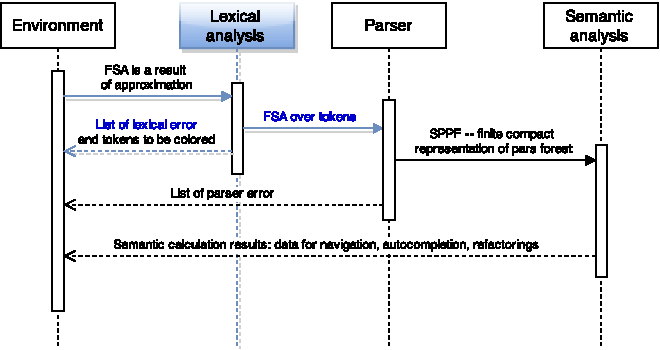
\includegraphics[width=0.9\textwidth]{Polubelova/Seq_with_lexer_highlighted}
\caption{Диаграмма последовательности, показывающая взаимодействие компонентов инструмента YaccConstructor}
\label{fig:seqYC} 
\end{center}
\end{figure}

\section{Алгоритм лексического анализа}

Основной задачей лексического анализа является выделение токенов во входном потоке символов, соответствующих спецификации обрабатываемого языка, и сохранение привязки лексических единиц к исходному коду. В классическом лексическом анализе входной поток является линейным, но для проведения лексического анализа динамически формируемого строкового выражения необходима структура, которая являлась бы компактным представлением множества значений этого выражения. Как уже было сказано, такие выражения получаются в результате строковых операций и языковых конструкций языка, с помощью которых эти строки и формируются. В данной работе такой структурой является конечный автомат, который можно представить в виде графа с отмеченными вершинами, соответствующие начальным и конечным состояниям исходного автомата, а ребра этого графа будут содержать строки\footnote{В дальнейшем для конечного автомата и для конечного преобразователя будет использоваться терминология, применимая к графам.}. 

В классическом лексическом анализе распространенной практикой является применение генераторов лексических анализаторов, которые по спецификации обрабатываемого языка строят описание конечного преобразователя. На основе него входной поток символов переводятся в поток токенов. Данный подход можно использовать и для лексического анализа динамически формируемых строковых выражений. 

Результатом работы лексического анализа динамически формируемого строкового выражения будет являться конечный автомат, каждое ребро которого содержит токен. В классическом лексическом анализе токен можно представить в виде структуры, содержащей идентификатор токена и последовательность символов, выделенной из входного потока. В нашем же случае токен будет представлять структуру, содержащую идентификатор токена  и \textit{конечный автомат}, который представляет собой часть множества значений исходного динамически формируемого строкового выражения, которая выделена лексическим анализатором в данный тип токена. При этом для каждого символа хранится информация, из какой строки получен этот символ и координаты его позиций внутри этой строки. 

Предлагаемый алгоритм для проведения лексического анализа динамически формируемого строкового выражения состоит из следующих шагов:

\textbf{\underline{Шаг 1}}. На вход лексическому анализатору подается конечный автомат, являющийся результатом аппроксимации динамически формируемого строкового выражения. Вершины графа соответствуют случаям конкатенации строк, наличие циклов в графе означает, что формирование строк происходило при участии языковых конструкций, например, \verb|for| и \verb|while|, ветвления в графе соответствуют условным операторам.  

\textbf{\underline{Шаг 2}}. Входной конечный автомат над строками преобразуется к конечному автомату над символами следующим образом: каждое ребро входного конечного автомата разбивается на последовательность новых ребер, метки которых содержат только по одному символу из строки исходного ребра. На этом этапе происходит сохранение привязки: с каждым символом сохраняются координаты позиций этого символа в исходной строке, а также привязка этой строки к исходному коду. Над полученным конечным автоматом запускаем процедуру построения детерминированного конечного автомата. 

\textbf{\underline{Шаг 3}}. Из конечного автомата, полученного на предыдущем шаге, строим конечный преобразователь следующим образом: для каждого ребра конечного автомата строим новое ребро конечного преобразователя, содержащее пару, первый аргумент которой содержит информацию, хранимую на ребре конечного автомата, то есть символ и его привязку к исходному коду, а второй аргумент {---} только этот символ.

\textbf{\underline{Шаг 4}}. Затем происходит применение операции композиция к двум конечным преобразователям, где первый конечный преобразователь получен на предыдущем шаге, а второй {---} из описания, построенного генератором лексических анализаторов, по спецификации обрабатываемого языка. Результатом этой операции является либо набор лексических ошибок, либо конечный преобразователь, каждое ребро которого содержит пару. Первым элементом этой пары является символ со свой привязкой к исходному коду, а вторым {---} функция, которая возвращает либо токен, либо ничего.

\textbf{\underline{Шаг 5}}. На этом шаге происходит интерпретация полученного конечного преобразователя, результатом которой будет являться конечный автомат над токенами.

При поддержке строковых операций особый интерес представляет строковая операция \verb|replace|$(M_1, M_2, M_3)$, где $M_1, M_2, M_3$ являются детерминированными конечными автоматами, так как поддержка ряда других часто используемых строковых операций может быть реализована на его основе. Конечные автоматы $M_1, M_2, M_3$ порождают языки $L(M_1), L(M_2), L(M_3)$ соответственно. \textbf{Replace} --- это операция, которая для любого слова из языка $L(M_1)$ ищет вхождения любого слова из языка $L(M_2)$ и заменяет их на слова из языка $L(M_3)$. Результатом строковой операции \verb|replace| является конечный автомат. При этом есть строковые операции, которые выводят обрабатываемый язык за класс регулярных и контекстно-свободных языков. 

Если строковые выражения формировались при участии строковых операций, которые можно выразить с помощью строковой операции \verb|replace|, то для их раскрытия требуется выполнение первых двух шагов описанного алгоритма для каждого участвующего в строковой операции конечного автомата. Далее применяется алгоритм, описанный в статье~\cite{ReplaceFangYu}. Но так как авторы этой статьи используют MBDD-представление для конечного автомата, а текущая реализация инструмента этого не предполагает, то алгоритм был упрощен и стал состоять из следующих шагов ($\#_1, \#_2 \notin \Sigma$, где $\Sigma$ --- входной алфавит конечных автоматов $M_1, M_2, M_3$): 

\textbf{\underline{Шаг 1}}. Построение конечного автомата $M'_1$ из $M_1$: дублируем состояния конечного автомата $M_1$, затем каждое исходное состояние соединяем с дублированным состоянием, соответствующее этому исходному состоянию, переходом по символу $\#_1$, а каждое дублированное состояние соединяем с исходным состоянием --- по символу~$\#_2$. То есть $L(M'_1) = \{ w' | k > 0, w =  w_{1}x_{1}w_{2}\ldots w_{k}x_{k}w_{k+1} \in L(M_1), w' = w_{1}\#_{1}x_{1}\#_{2}w_{2}\ldots w_{k}\#_{1}x_{k}\#_{2}w_{k+1}\}$.

\textbf{\underline{Шаг 2}}. Построение конечного автомата $M'_2$ из $M_2$. Для начала построим конечный автомат $M_h$, который принимает строки, не содержащие в себе любую подстроку из языка $L(M_2)$.  То есть $L(M_h)$ является дополнением к множеству $\{w_{1}xw_{2} | x \in L(M_2), w_1, w_2 \in \Sigma^{\star}\}$. Затем соединим конечные состояния конечного автомата $M_h$ с начальным состоянием конечного автомата $M_2$ по символу $\#_1$, а также конечные состояния конечного автомата $M_2$ с начальным состоянием конечного автомата $M_h$ по символу $\#_2$. То есть $L(M'_2) = \{ w' | k > 0, w' = w_{1}\#_{1}x_{1}\#_{2}w_{2} \ldots w_{k}\#_{1}x_{k}\#_{2}w_{k+1}, \forall 1 \le i \le k, x_i \in L(M_2), \forall 1 \le i \le k+1, w_i \in L(M_h)\}$.

\textbf{\underline{Шаг 3}}. Построение конечного автомата $M'$ как результат операции пересечения над конечными автоматами $M'_1$ и $M'_2$.

\textbf{\underline{Шаг 4}}. Результирующий конечный автомат $M$ получается из конечного автомата $M'$ путем замены строк, которые находятся между символами $\#_1$ и $\#_2$, на слова языка $L(M_3)$. То есть $L(M) = \{ w | k > 0, w_{1}\#_{1}x_{1}\#_{2}w_{2}\ldots w_{k}\#_{1}x_{k}\#_{2}w_{k+1} \in L(M'_1) \cap L(M'_2), w = w_{1}c_{1}w_{2}\ldots w_{k}c_{k}w_{k+1} \forall 1 \le i \le k, c_i \in L(M_3)\}$.

После раскрытия операции \verb|replace| можно продолжить выполнение алгоритма для проведения лексического анализа строкового выражения со следующего шага. 

Рассмотрим следующий пример кода:

\fvset{frame=lines,framesep=5pt}
\begin{listing}[H]
    \begin{lstlisting}[language=csharp]
 private void Go(int cond){
   string columnName = cond > 3 ? "X" : (cond < 0 ? "Y" : "Z");
   string queryString = "SELECT name" + columnName + " FROM table";
   Program.ExecuteImmediate(queryString);}
    \end{lstlisting}
\caption{Пример кода}
\label{lst:example1}
\end{listing}

Результатом аппроксимации этого кода будет конечный автомат (см рис.~\ref{fig:example_appr}).

\begin{figure}[H]
\begin{center}
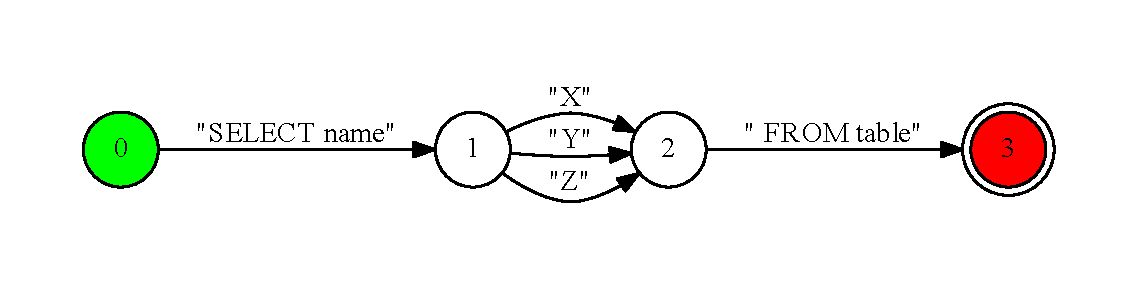
\includegraphics[width=0.75\textwidth]{Polubelova/tsql_test}
\caption{Результат аппроксимации кода, представленного в листинге~\ref{lst:example1}}
\label{fig:example_appr} 
\end{center}
\end{figure}

Конечный автомат, полученный в результате применения описанного выше алгоритма лексического анализа динамически формируемого строкового выражения к конечному автомату, представленного на рис.~\ref{fig:example_appr}, показан на рис.~\ref{fig:example_lexer}.

\begin{figure}[h!]
\begin{center}
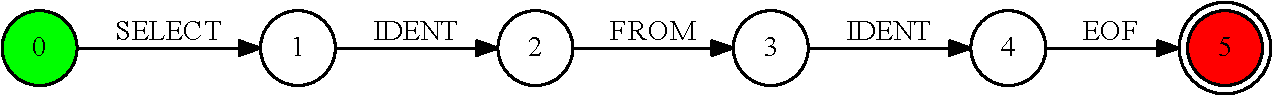
\includegraphics[width=0.9\textwidth]{Polubelova/tsql_test_appr}
\caption{Результат работы лексера для конечного автомата, представленного на рис.~\ref{fig:example_appr}}
\label{fig:example_lexer} 
\end{center}
\end{figure}

При этом токен \verb|SELECT| содержит в себе конечный автомат, представленный на рис.~\ref{fig:tsql_select}. Конечный автомат первого токена \verb|IDENT| представлен на рис.~\ref{fig:tsql_ident_1}. Второго токена \verb|IDENT| --- на рис.~\ref{fig:tsql_ident_2}. Видно, что для каждого символа сохраняются строка, из которой этот символ получен, и координаты этого символа внутри этой строки. Так как токен содержит в себе конечный автомат, а не строку, то получается один идентификатор \verb|IDENT| после \verb|SELECT|, а не три, как это было раньше~\cite{Verbitskaya, Polubelova}, что упрощает проведение синтаксического разбора в таких случаях.  

\begin{figure}[H]
\begin{center}
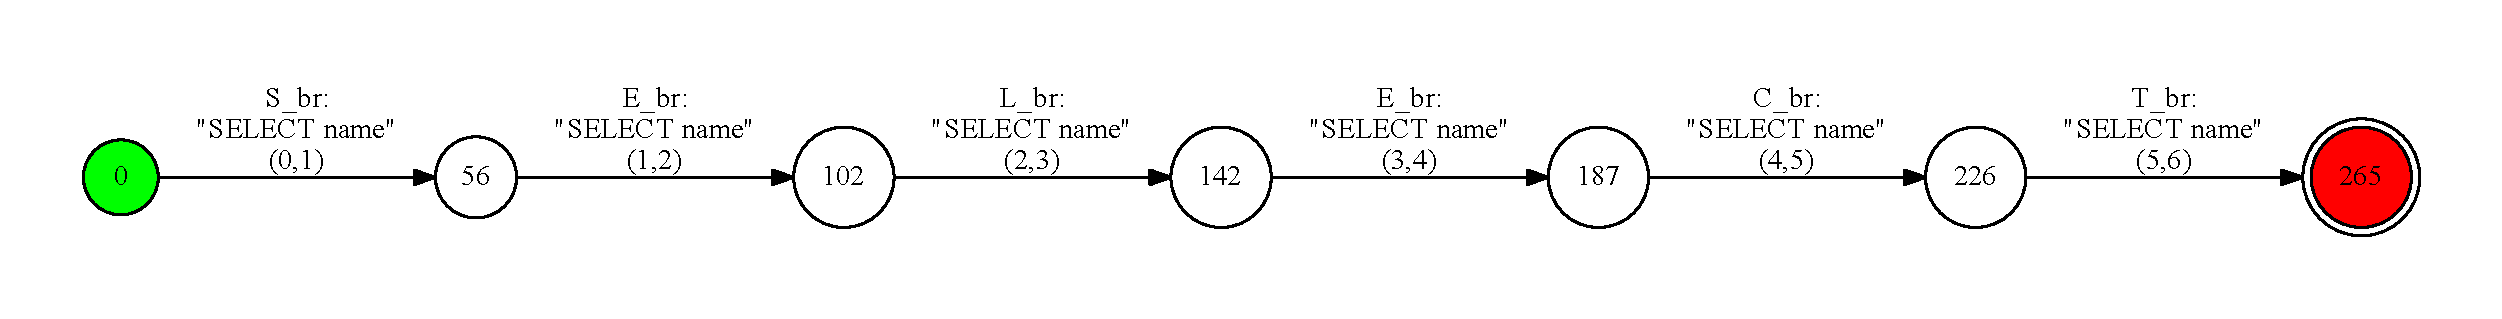
\includegraphics[width=1.0\textwidth]{Polubelova/tsql_select}
\caption{Конечный автомат, содержащейся в токене SELECT}
\label{fig:tsql_select} 
\end{center}
\end{figure}

\begin{figure}[H]
\begin{center}
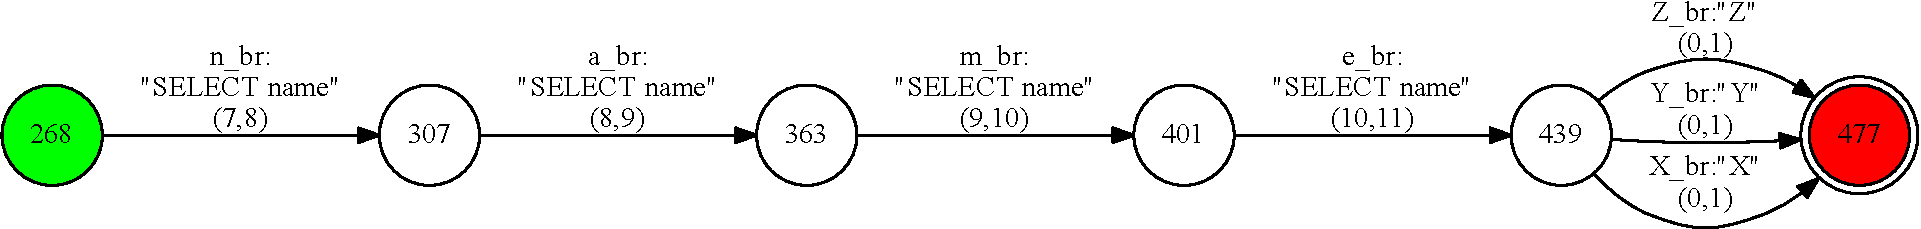
\includegraphics[width=1.0\textwidth]{Polubelova/tsql_ident_1}
\caption{Конечный автомат, содержащейся в первом токене IDENT}
\label{fig:tsql_ident_1} 
\end{center}
\end{figure}

\begin{figure}[H]
\begin{center}
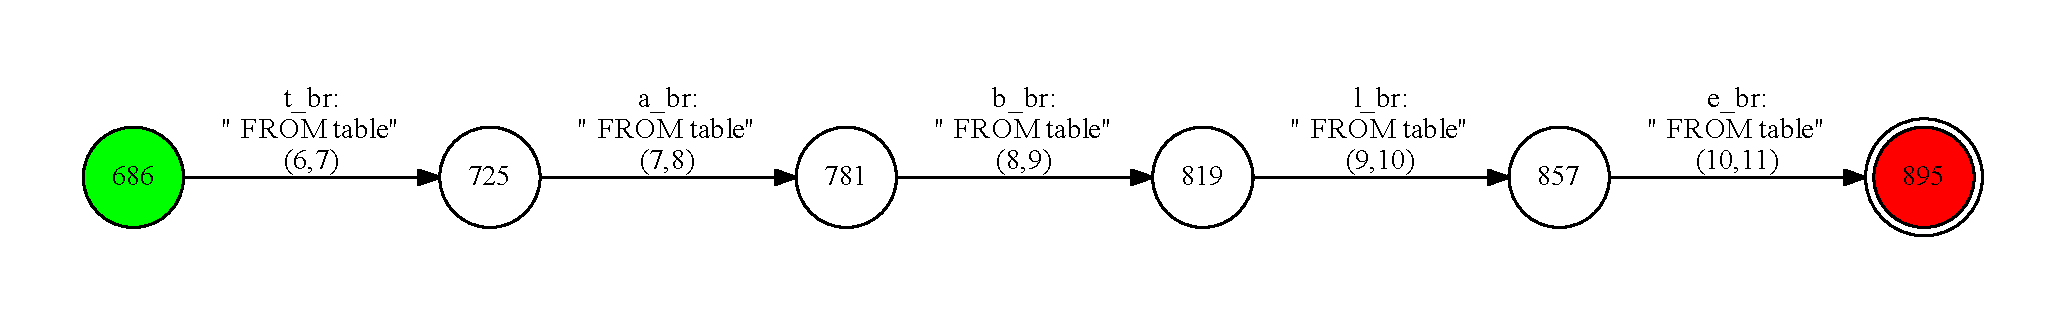
\includegraphics[width=1.0\textwidth]{Polubelova/tsql_ident_2}
\caption{Конечный автомат, содержащейся во втором токене IDENT}
\label{fig:tsql_ident_2} 
\end{center}
\end{figure}


\section{Особенности реализации}

\subsection{Архитектура инструмента}

В рамках проекта YaccConstructor была создана и реализована архитектура инструмента, реализующая алгоритм для проведения лексического анализа динамически формируемых строковых выражений. Диаграмма компонентов реализованного инструмента представлена на рис.~\ref{fig:CompDiag}.

\begin{figure}[h!]
\begin{center}
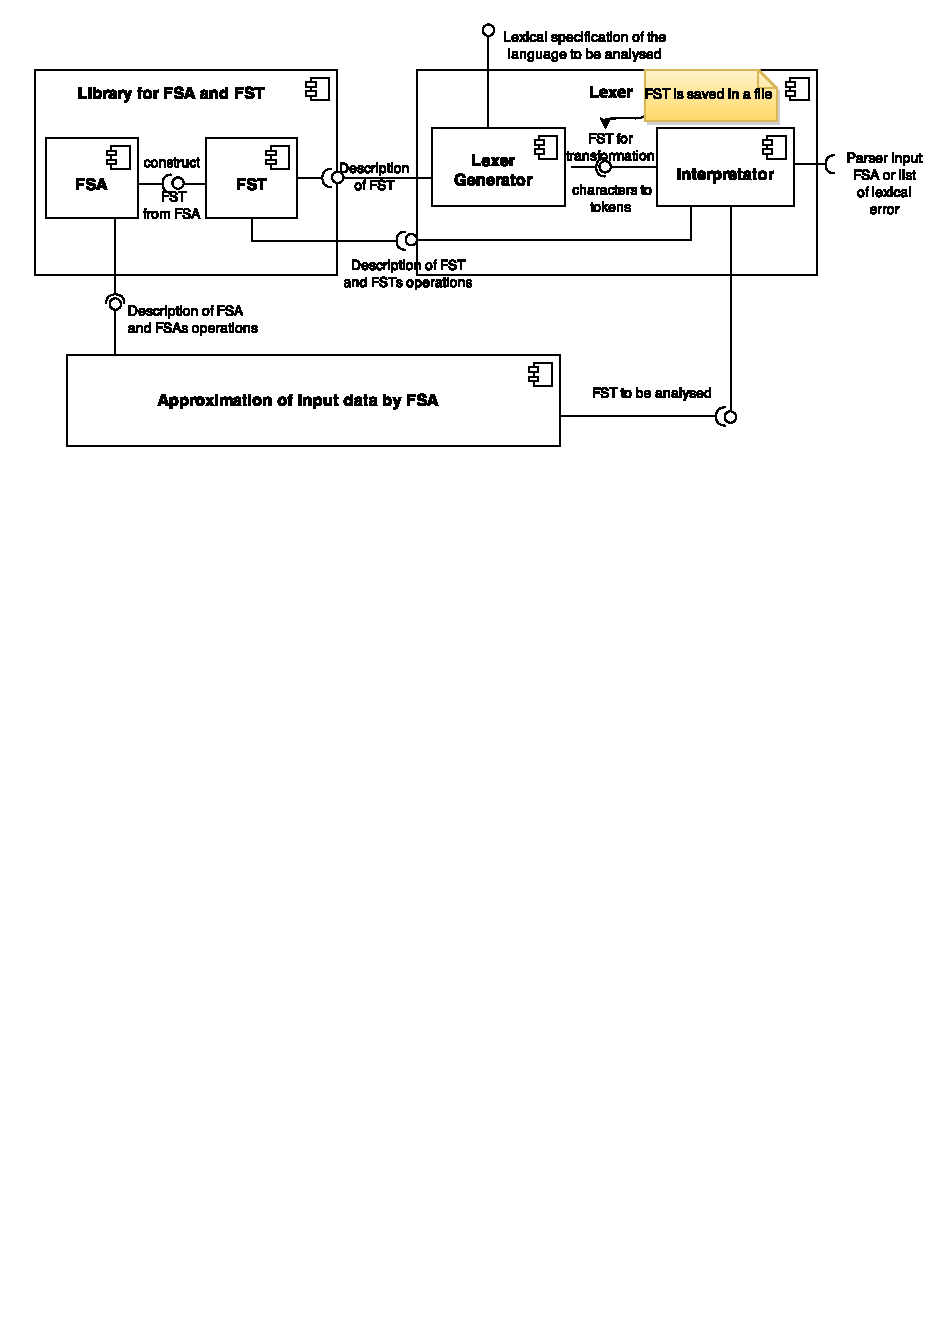
\includegraphics[width=1.0\textwidth]{Polubelova/ComponentDiagram}
\caption{Диаграмма компонентов реализованного инструмента}
\label{fig:CompDiag} 
\end{center}
\end{figure}

Ниже представлено описание каждого компонента. 

Компонент \textbf{Approximation of input data by FSA} отвечает за аппроксимацию входного динамически формируемого строкового выражения, результатом которой будет конечный автомат. Для реализации этого компонента нужно знать описание конечного автомата и иметь доступ к операциям над ними. Например, при раскрытии операции \verb|Replace| потребуется вызов соответствующей функции в библиотеке (компонент \textbf{Library for FSA and FST}). 

Компонент \textbf{Library for FSA and FST} состоит из двух компонентов: \textbf{FSA} (Finite State Automata) и \textbf{FST} (Finite State Transducer), которые являются библиотеками для конечного автомата и конечного преобразователя соответственно. Библиотека для конечного автомата используется для построения аппроксимации входных данных, а библиотека для конечных преобразователей --- для проведения лексического анализа динамически формируемых строковых выражений. Диаграмма классов этой библиотеки представлена на рис.~\ref{fig:ClassLib}. Для конечного автомата реализовано ряд операций таких как: пересечение, объединение, дополнение, конкатенация, Replace, построение детерминированного конечного автомата из недетерминированного. Для конечного преобразователя реализованы операции композиция, объединение, пересечение и построение конечного преобразователя из конечного автомата с помощью функции преобразования. Язык реализации библиотеки --- F\#. Для представления конечного автомата и конечного преобразователя в виде графа, ребра которого соответствуют переходам, а вершины --- состояниям, использовалась библиотека QuickGraph~\cite{QuickGraph}. Для их визуализации --- инструмент Graphviz~\cite{Graphviz}.

Компонент \textbf{Lexer} состоит из двух компонентов: \textbf{Lexer Generator} и \textbf{Interpretator}, которые являются генератором лексических анализаторов и лексическим анализатором соответственно. За основу генератора лексических анализаторов для динамически формируемых строковых выражений взят инструмент FsLex, который по спецификации обрабатываемого языка строит описание конечного преобразователя. Генератор лексических анализаторов FsLex был изменен так, чтобы он строил описание конечного преобразователя, соответствующее реализованной библиотеки (компонент \textbf{Library for FSA and FST}). При этом это описание сохраняется в отдельном файле, что позволяет многократно использовать описание конечного преобразователя для обработки одного языка. Лексический анализатор на вход принимает два конечных преобразователя. Первый преобразователь получен в результате преобразования конечного автомата, являющейся результатом аппроксимации обрабатываемого входного динамически формируемого строкового выражения (компонент \textbf{Approximation of input data by FSA}), а второй преобразователь взят из описания, построенного генератором лексических анализаторов. Результатом работы лексического анализатора будет являться либо конечный автомат над токенами, либо список лексических ошибок. Диаграмма классов этого компонента представлена на рис.~\ref{fig:ClassLexer}. Язык реализации лексера --- F\#.

\begin{figure}[h!]
\begin{center}
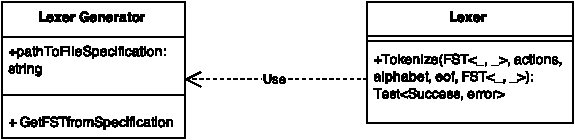
\includegraphics[width=0.8\textwidth]{Polubelova/ClassDiagramLexer}
\caption{Диаграмма классов компоненты \textbf{Lexer}}
\label{fig:ClassLexer} 
\end{center}
\end{figure}

\begin{figure}[h!]
\begin{center}
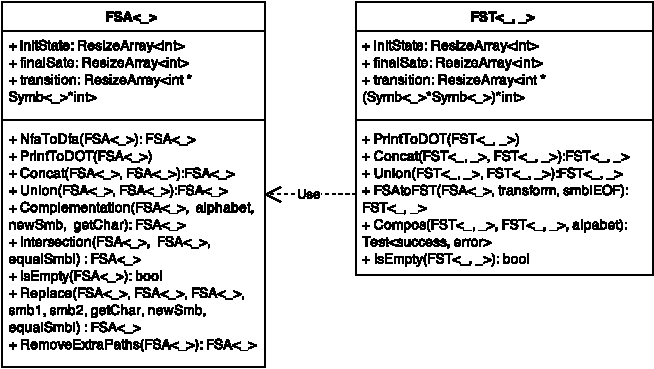
\includegraphics[width=1.0\textwidth]{Polubelova/ClassDiagramLib}
\caption{Диаграмма классов компоненты \textbf{Library for FSA and FST} }
\label{fig:ClassLib} 
\end{center}
\end{figure}


\subsection{Детали реализации}

\subsubsection{Конечные автоматы}

Результатом некоторых операций над конечными автоматами, например, пересечение, может быть пустой конечный автомат. \textit{Пустым конечным автоматом} будем называть граф, у которого не существует пути от начального состояния до какого-либо конечного состояния. Полагаем, что конечный автомат, не содержащий переходов и имеющий только одно состояние, в котором начальное состояние совпадает с конечным, принимает \textit{пустой} язык, но при этом этот автомат не является пустым, так как существует путь от начального состояния до конечного состояния длины 0. 

В конечном автомате могут существовать ``ненужные'' состояния, то есть состояния, которые не лежат на пути от начального состояния до какого-либо конечного состояния. Алгоритм для удаления таких состояний состоит из следующих шагов:

\textbf{\underline{Шаг 1}}. Считаем, что у конечного автомата только одно начальное состояние. Если конечных состояний несколько, то добавляем одно новое состояние и переходы по \verb|Eps| к этому состоянию от каждого конечного состояния. Считаем добавленное состояние конечным, то есть получаем одно конечное состояние.

\textbf{\underline{Шаг 2}}. Запускаем обход в глубину (Depth-first search, dfs) от начальной вершины над конечным автоматом, полученным на предыдущем шаге. Удаляем не посещенные вершины из множества всех состояний и из конечных состояний (исходного конечного автомата).

\textbf{\underline{Шаг 3}}. Создаем новый конечный автомат, который отличается от текущего конечного автомата тем, что ребра имеют другое направление. То есть получаем инвертированный конечный автомат.

\textbf{\underline{Шаг 4}}. Запускаем обход в глубину от конечной вершины над конечным автоматом, полученным на предыдущем шаге. Удаляем не посещенные вершины из множества всех состояний и из начального состояния (исходного конечного автомата). 

\textbf{\underline{Шаг 5}}. Удаляем состояние, которое было добавлено на Шаге 1. 

Данный алгоритм можно использовать для входного конечного автомата, прежде чем над ним будут проводить какие-либо операции, что позволит сократить количество состояний в этом конечном автомате.

Для того чтобы узнать, является ли конечный автомат пустым, достаточно будет запустить обход в глубину от стартовой вершины и проверить, все ли конечные состояния лежат в множестве не посещенных состояний.

Если в операции \verb|Replace|$(M_1, M_2, M_3)$ над конечными автоматами хотя бы один конечный автомат является пустым, то результатом будет являться конечный автомат~$M_1$. Результат операции \verb|Replace|, в которой хотя бы один аргумент является конечный автомат с одним состоянием, являющимся и конечным и начальным, и без переходов, представлен ниже.

Пусть $M_1$ --- есть конечный автомат с одним состоянием, являющимся и начальным и конечным, и без переходов. Если $M_2$ --- конечный автомат, который содержит пустое слово, то \verb|Replace|$(M_1, M_2, M_3) = M_3$, иначе \verb|Replace|$(M_1, M_2, M_3) = M_1$. 

Если $M_2$ --- есть конечный автомат с одним состоянием, являющимся и начальным и конечным, и без переходов, то во все состояния конечного автомата $M_1$ вставляем конечный автомат $M_3$. 

\subsubsection{Лексический анализ}

В алгоритме лексического анализа строковых выражений присутствует этап интерпретации конечного преобразователя (\textbf{Шаг 5}), полученного в результате операции композиция над двумя конечными преобразователями. Рассмотрим этот процесс более подробно. 

Пусть дан входной конечный автомат, представленный на рис.~\ref{fig:calc_ex}.

\begin{figure}[H]
\begin{center}
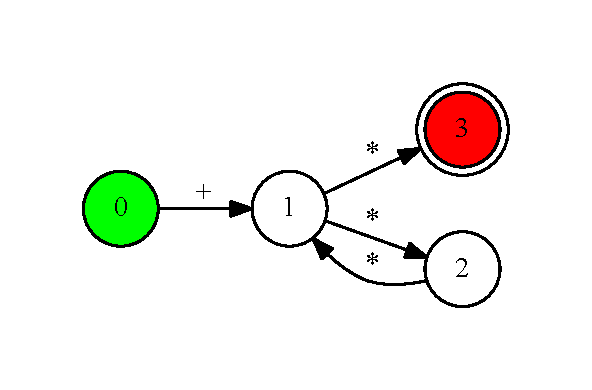
\includegraphics[width=0.28\textwidth]{Polubelova/calc_ex}
\caption{Входной конечный автомат}
\label{fig:calc_ex} 
\end{center}
\end{figure}
Результат композиции конечного преобразователя (преобразованный конечный автомат, \textbf{Шаг 3}) с конечным преобразователем, полученным из описания, построенным генератором лексического анализатора по спецификации языка для калькулятора (см. листинг~\ref{lst:calc}), представлен на рис.~\ref{fig:calc_ex_compose}. Где 6 --- номер функции, которую возвращает токен \verb|PLUS|, 7 --- номер функции, которую возвращает токен \verb|POW|, 8 --- номер функции, которую возвращает токен \verb|MULT|.

\fvset{frame=lines,framesep=5pt}
\begin{listing}[H]
    \begin{lstlisting}[language=csharp,numbers=none]
let digit = ['0'-'9']
let whitespace = [' ' '\t' '\r' '\n']

rule token = parse
| whitespace { None }
| digit+ ('.'digit+)? (['e' 'E'] digit+)? { NUMBER(gr) |> Some }
| '-' { MINUS(gr) |> Some }
| '(' { LBRACE(gr) |> Some }
| ')' { RBRACE(gr) |> Some }
| '/' { DIV(gr)|> Some }
| '+' { PLUS(gr)|> Some }
| "**" { POW(gr)|> Some }
| '*' { MULT(gr)|> Some }
    \end{lstlisting}
\caption{Спецификация языка для калькулятора}
\label{lst:calc}
\end{listing}

\begin{figure}[h!]
\begin{center}
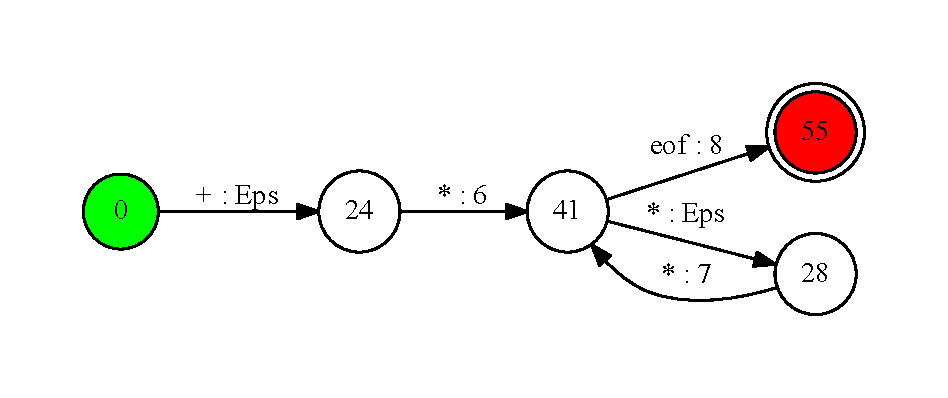
\includegraphics[width=0.6\textwidth]{Polubelova/calc_ex_compose}
\caption{Результат операции композиция}
\label{fig:calc_ex_compose} 
\end{center}
\end{figure}
Для каждого токена сохраняется конечный автомат, который представляет собой часть множества значений исходного динамически формируемого строкового выражения, которая выделена лексическим анализатором в данный тип токена. Чтобы это сделать, необходима структура \verb|GraphAction|, которая хранит одну стартовую action-вершину и несколько конечных action-вершин, а также конечный автомат. \textit{Стартовая action-вершина} --- это вершина, из которой выходит ребро, содержащее номер функции. \textit{Конечные action-вершины} --- это вершины, в которых заканчивается обход в ширину (Breadth-first search, bfs) из стартовой action-вершины. Условием окончания является встреча action-вершины или вершины, принадлежащей множеству конечных или стартовых состояний. Конечный автомат хранит результат графа, посещенный обходом в ширину. Алгоритм получения конечного автомата для каждого токена представлен ниже.

\textbf{\underline{Шаг 1}}. Для конечного преобразователя получаем набор вершин, которые являются стартовыми action-вершинами. Считаем также, что начальное состояние конечного автомата входит в стартовую action-вершину. Запускаем обход в ширину для каждой стартовой action-вершины, который ищет конечные action-вершины. Полученный результат сохраняем в структуре \verb|GraphAction|.  

\textbf{\underline{Шаг 2}}. Создаем новый конечный преобразователь, который получается путем инвертирования ребер исходного конечного преобразователя. Для этого преобразователя также получаем набор вершин, которые являются стартовыми action-вершинами. Конечное состояние также входит в множество стартовых action-вершин. Запускаем обход в ширину для каждой стартовой action-вершины, который ищет конечные action-вершины. Полученный результат сохраняем в структуре \verb|GraphAction|. 

\textbf{\underline{Шаг 3}}. Для каждой структуры \verb|GraphAction|, полученной на Шаге 1, и для каждой конечной  action-вершины этой структуры ищем соответствующую структуру \verb|GraphAction|, полученную на Шаге 2, в которой стартовая action-вершина совпадает с текущей конечной action-вершиной. Учитывая, что во второй структуре ребра являются инвертированными, относительно исходного конечного преобразователя, ищем пересечение двух конечных преобразователей. Результатом будет являться токен, идентификатор которого есть номер функции, которую возвращает конечная action-вершина, а также конечный автомат, полученный в результате пересечения (оставив только первые аргументы результата пересечения двух конечных преобразователей), в котором начальное состояние совпадает со стартовой action-вершиной, а конечное --- с множеством конечных action-вершин. При этом в конечный автомат, являющейся результатом лексического анализа, добавляется ребро, содержащее этот токен, исходная вершина которого равна стартовой action-вершины, а целевая вершина --- текущей конечной action-вершины. 

Для рассмотренного примера стартовыми action-вершинами являются следующие вершины: 0, 24, 28, 41. Построим для каждой из них структуру \verb|GraphAction| (см. таблицу~\ref{tbl:GraphAction}). 

\begin{table}[h]
  \centering
  \begin{tabular}{ | c | c | c | c | }
    \hline
    0 & 24 & 28 & 41 \\ \hline
    \begin{minipage}{.22\textwidth}
      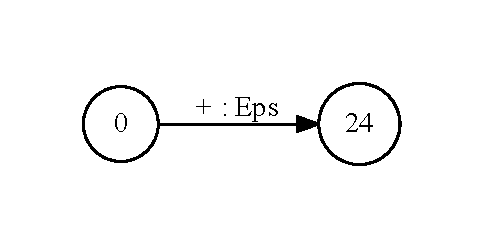
\includegraphics[width=\linewidth]{Polubelova/0_tok}
    \end{minipage}
    &
    \begin{minipage}{.22\textwidth}
      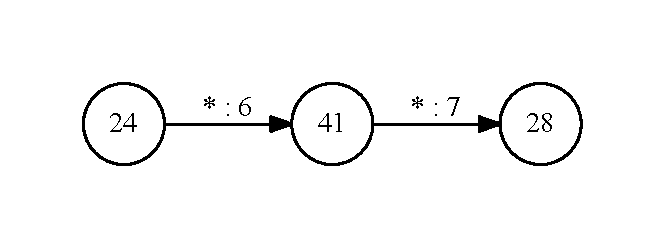
\includegraphics[width=\linewidth]{Polubelova/24_tok}
    \end{minipage}
    & 
    \begin{minipage}{.22\textwidth}
      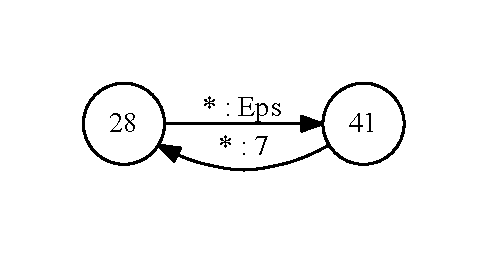
\includegraphics[width=\linewidth]{Polubelova/28_tok}
    \end{minipage}
    & 
    \begin{minipage}{.22\textwidth}
      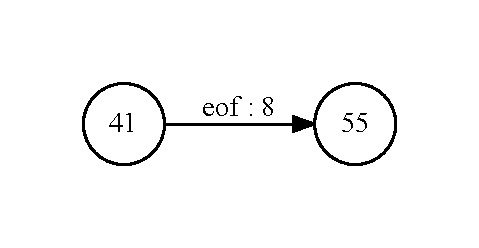
\includegraphics[width=\linewidth]{Polubelova/41_tok}
    \end{minipage}    
    \\ \hline
    24 & 41, 28 & 28, 41 & 55
    \\ \hline
  \end{tabular}
  \caption{Структура GraphAction для Шага 1}
  \label{tbl:GraphAction}
\end{table}

Результат выполнения Шага 2 представлен в таблице~\ref{tbl:GraphActionInv}. При этом конечный автомат показан инвертированным. Также для этого шага не важно, какие конечные action-вершины получаются.

\begin{table}[h]
  \centering
  \begin{tabular}{ | c | c | c | c | }
    \hline
    24 & 28 & 41 & 55 \\ \hline
    \begin{minipage}{.22\textwidth}
      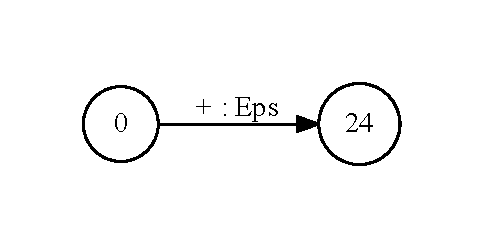
\includegraphics[width=\linewidth]{Polubelova/24_inv}
    \end{minipage}
    &
    \begin{minipage}{.22\textwidth}
      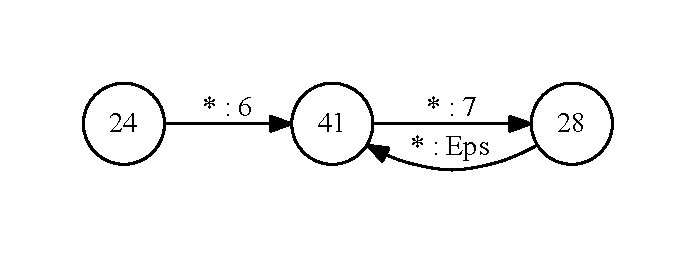
\includegraphics[width=\linewidth]{Polubelova/28_inv}
    \end{minipage}
    & 
    \begin{minipage}{.22\textwidth}
      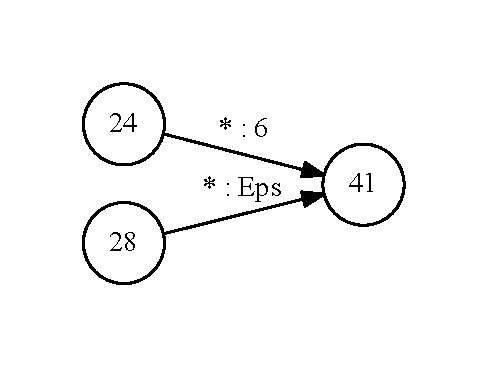
\includegraphics[width=\linewidth]{Polubelova/41_inv}
    \end{minipage}
    & 
    \begin{minipage}{.22\textwidth}
      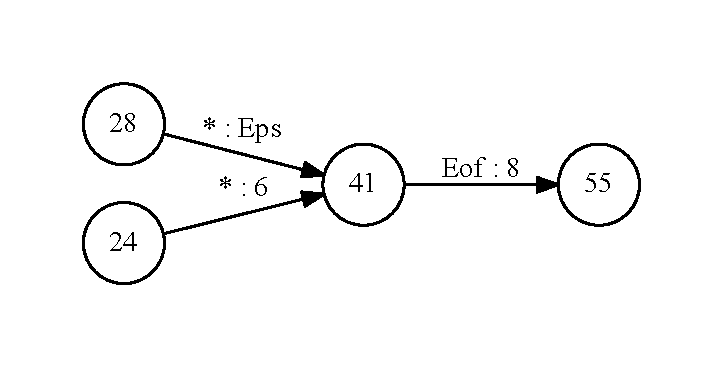
\includegraphics[width=\linewidth]{Polubelova/55_inv}
    \end{minipage}    
    \\ \hline
  \end{tabular}
  \caption{Структура GraphAction для Шага 2}
  \label{tbl:GraphActionInv}
\end{table}

Результат пересечения двух конечных преобразователей, один из которых взят из таблицы~\ref{tbl:GraphAction}, а второй --- из таблицы~\ref{tbl:GraphActionInv}, при условии что стартовая action-вершина второго конечного преобразователя совпадает с текущей конечной action-вершиной, представлен в таблице~\ref{tbl:GraphActionInters}.

\begin{table}[h]
  \centering
  \begin{tabular}{ | c | c | c |}
    \hline
    \begin{minipage}{.3\textwidth}
      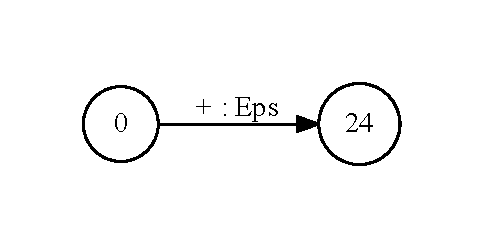
\includegraphics[width=\linewidth]{Polubelova/0_int}
    \end{minipage}
    &
    \begin{minipage}{.3\textwidth}
      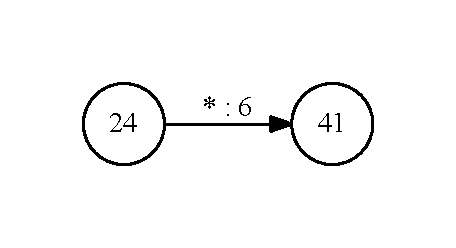
\includegraphics[width=\linewidth]{Polubelova/24_int}
    \end{minipage}
    & 
    \begin{minipage}{.3\textwidth}
      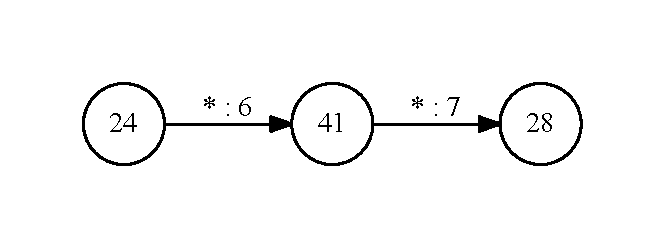
\includegraphics[width=\linewidth]{Polubelova/24_1_int}
    \end{minipage}
    \\ \hline
    \begin{minipage}{.3\textwidth}
      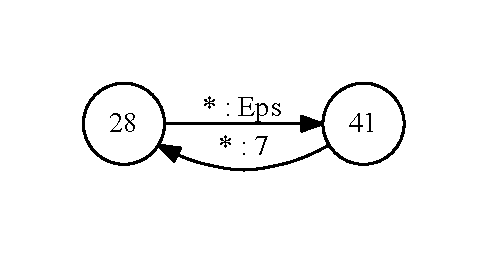
\includegraphics[width=\linewidth]{Polubelova/28_int}
    \end{minipage}
    &
    \begin{minipage}{.3\textwidth}
      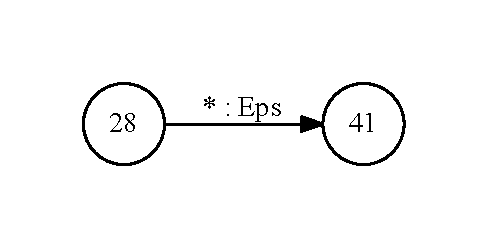
\includegraphics[width=\linewidth]{Polubelova/28_1_int}   
    \end{minipage}
    & 
    \begin{minipage}{.3\textwidth}
      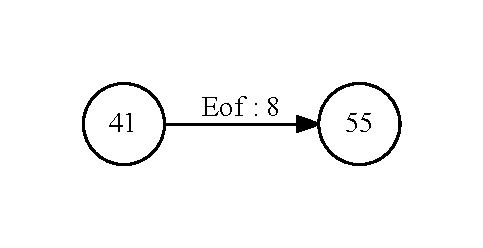
\includegraphics[width=\linewidth]{Polubelova/41_int}
    \end{minipage}
    \\ \hline
  \end{tabular}
  \caption{Результат пересечения конечных преобразователей из таблиц~\ref{tbl:GraphAction} и ~\ref{tbl:GraphActionInv}}
  \label{tbl:GraphActionInters}
\end{table}

Результатом лексического анализа конечного автомата, представленного на рис.~\ref{fig:calc_ex}, показан на рис.~\ref{fig:calc_ex_res}. 

\begin{figure}[h!]
\begin{center}
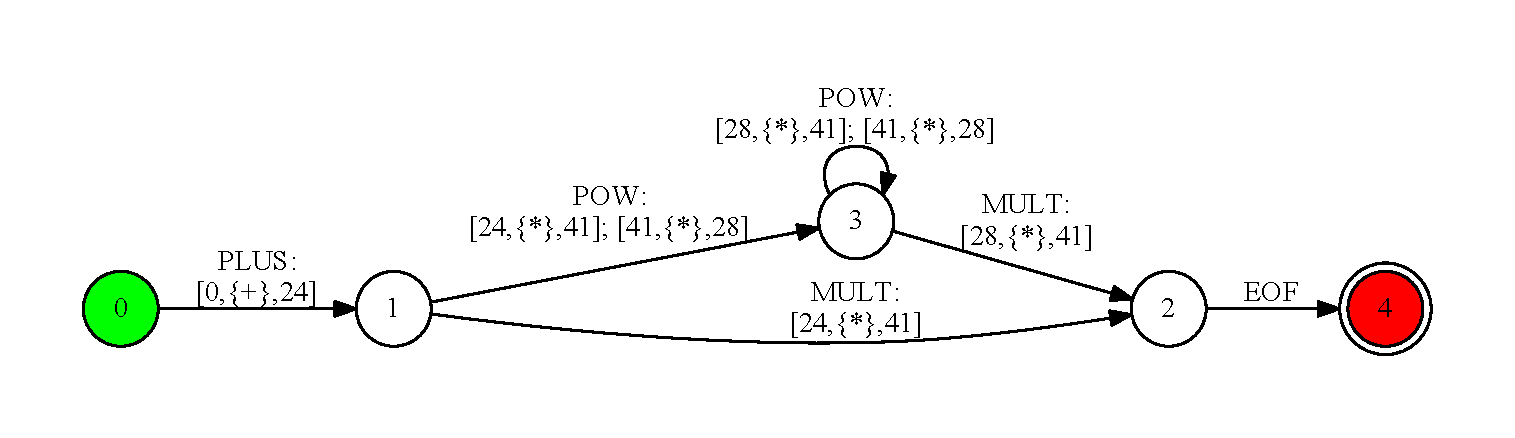
\includegraphics[width=1.0\textwidth]{Polubelova/calc_ex_res}
\caption{Результат лексического анализа}
\label{fig:calc_ex_res} 
\end{center}
\end{figure}


\section{Апробация}

Для данной апробации были подготовлены тесты, на которых реализованный инструмент выполняет поставленную перед ним задачу: обрабатывает случаи, когда строковые выражения были сформированы при участии циклов и строковых операций. Опишем основные этапы сценария тестирования:

\textbf{\underline{Этап 1}}. Описать спецификацию обрабатываемого языка в файле с расширением .fsl. Генератор лексических анализаторов по этой спецификации построит описание конечного преобразователя. 

\textbf{\underline{Этап 2}}. Создать проект, в который добавляем файл с описанием конечного преобразователя. Необходимо также будет описать тип \verb|Token|. 

\textbf{\underline{Этап 3}}. Для тестирования не важно, каким способом получены входные конечные автоматы. Главное, чтобы они удовлетворяли внутреннему описанию конечного автомата. 

\textbf{\underline{Этап 4}}. Когда входные конечные автоматы получены, можно выбрать проводимую операцию над ними. Это может быть, например, обработка операции \verb|replace|, результатом которой является также конечный автомат. Если все необходимые операции уже выполнены, то можно проводить лексический анализ. Для этого необходимо преобразовать конечный автомат в конечный преобразователь. Затем вызвать функцию \verb|tokenize| из сгенерированного файла. В случае успешного проведения лексического анализа, результат запишется в файл с расширением .dot, в котором будет описание конечного автомата над токенами. При этом для каждого токена можно распечатать хранимый им конечный автомат.

Рассмотрим примеры, которые показывают важность включения обработки строковых операций и циклов в проводимый анализ.  

\textbf{\underline{Пример 1}}. 
Рассмотрим следующий пример кода:
\fvset{frame=lines,framesep=5pt}
\begin{listing}[H]
    \begin{lstlisting}[language=csharp]
 private void Go(){
   String s = "SELECT nameX FROM tableY";
   s = s.Replace("SELECT nameX", "b");
   Program.ExecuteImmediate(s);
 }
    \end{lstlisting}
\caption{Пример кода cо строковой операцией Replace}
\label{lst:exampleR}
\end{listing}

В результате выполнения метода \verb|Replace| в переменной \verb|s| будет содержаться строка \textit{``b FROM tableY''}, что приведет к ошибке во время выполнения запроса. 

Результат лексического анализа с поддержкой строковой операцией \verb|Replace| представлен на рис.~\ref{fig:replace_ex_1}. Без поддержки --- на рис.~\ref{fig:replace_ex}.  

\begin{figure}[h!]
\begin{center}
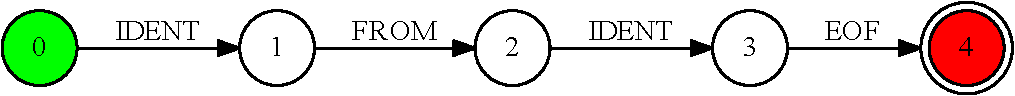
\includegraphics[width=0.7\textwidth]{Polubelova/ReplaceEx}
\caption{Результат лексического анализа с поддержкой строковой операцией Replace}
\label{fig:replace_ex_1} 
\end{center}
\end{figure}

\begin{figure}[h!]
\begin{center}
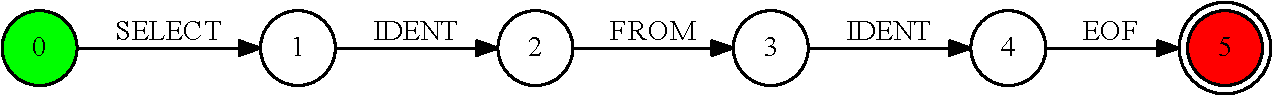
\includegraphics[width=0.8\textwidth]{Polubelova/ReplaceEx1}
\caption{Результат лексического анализа без поддержки строковой операцией Replace}
\label{fig:replace_ex} 
\end{center}
\end{figure}

\textbf{\underline{Пример 2}}. 
Рассмотрим следующий пример кода:
\fvset{frame=lines,framesep=5pt}
\begin{listing}[H]
    \begin{lstlisting}[language=csharp]
 private void Go(int number){
   String s = "SELECT nameX FROM tableY WHERE x < ";
   while(s.Length < number){ s += "+ 1 ";}
   Program.ExecuteImmediate(s);
 }
    \end{lstlisting}
\caption{Пример кода с циклом while}
\label{lst:exampleW}
\end{listing}

Результатом аппроксимации кода будет конечный автомат, представленный на рис.~\ref{fig:while_appr}. Результат лексического анализа представлен на рис.~\ref{fig:while_ex}.

\begin{figure}[h!]
\begin{center}
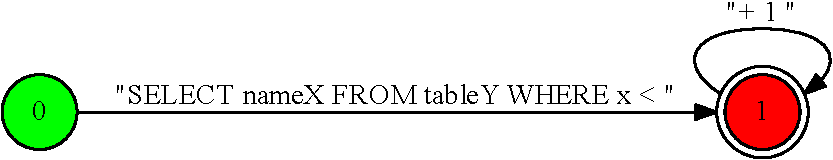
\includegraphics[width=0.75\textwidth]{Polubelova/while_appr}
\caption{Результат аппроксимации кода}
\label{fig:while_appr} 
\end{center}
\end{figure}


\begin{figure}[h!]
\begin{center}
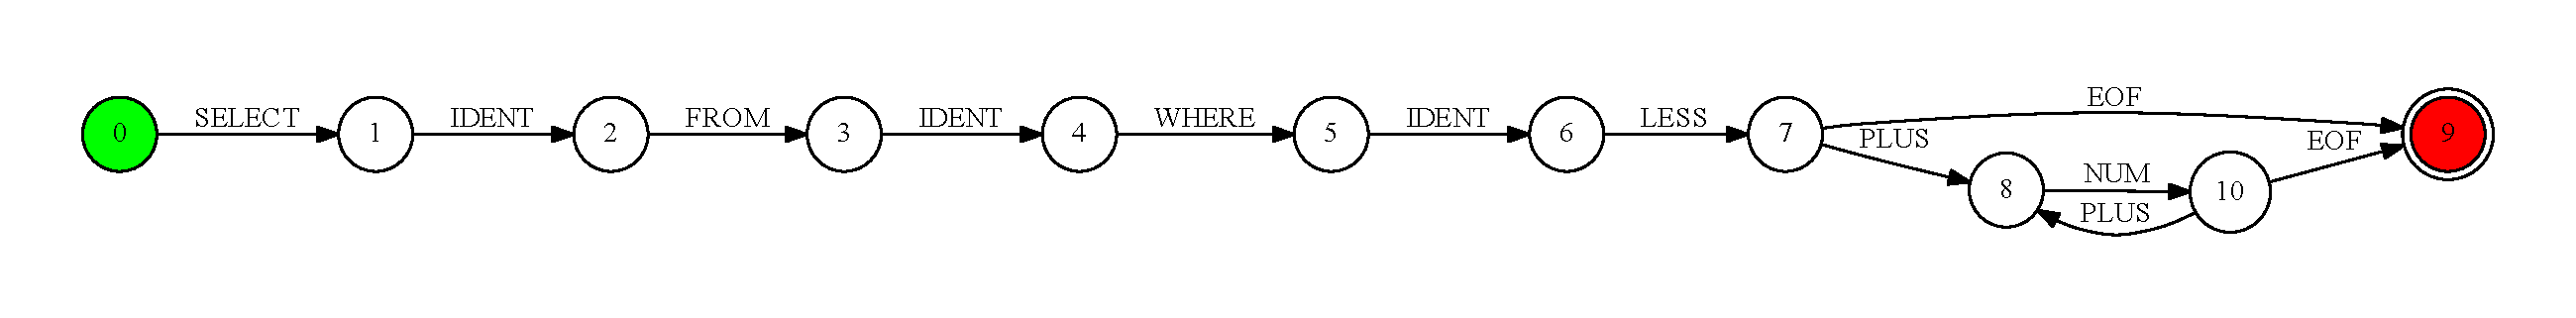
\includegraphics[width=1.0\textwidth]{Polubelova/WhileEx}
\caption{Результат лексического анализа с поддержкой циклов}
\label{fig:while_ex} 
\end{center}
\end{figure}

\textbf{\underline{Пример 3}}. 
Рассмотрим следующий пример кода, в котором конечный автомат токена содержит цикл:

\fvset{frame=lines,framesep=5pt}
\begin{listing}[H]
    \begin{lstlisting}[language=csharp]
   String s = "SELECT name";
   for(int i = 0; i < 10; i++){ s += "X";}
   s+= " FROM tableY";
   Program.ExecuteImmediate(s);
    \end{lstlisting}
\caption{Пример кода, в котором конечный автомат токена содержит цикл}
\label{lst:example}
\end{listing}

Результат лексического анализа будет конечный автомат, представленный на рис.~\ref{fig:TokenEx}. Конечный автомат первого токена \verb|IDENT|, содержащий цикл, представлен на рис.~\ref{fig:token}. На этом же рисунке показана сохраненная привязка символов к исходному коду. 

\begin{figure}[h!]
\begin{center}
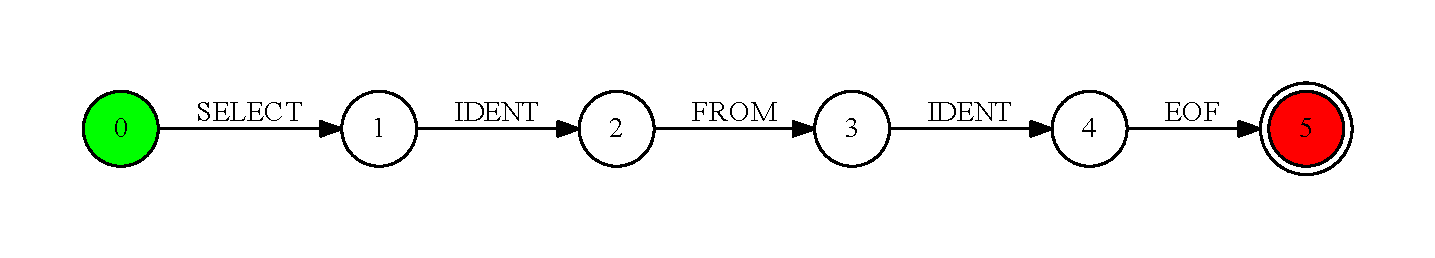
\includegraphics[width=1.0\textwidth]{Polubelova/TokenEx}
\caption{Результат лексического анализа}
\label{fig:TokenEx} 
\end{center}
\end{figure}

\begin{figure}[h!]
\begin{center}
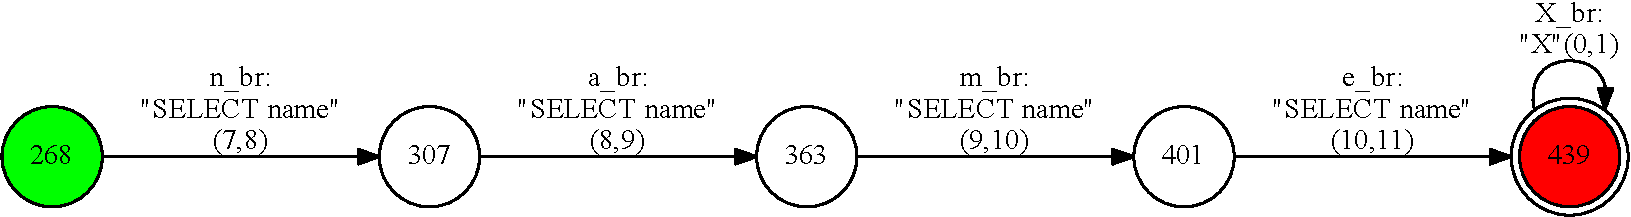
\includegraphics[width=1.0\textwidth]{Polubelova/token}
\caption{Конечный автомат первого токена IDENT, содержащий цикл}
\label{fig:token} 
\end{center}
\end{figure}


%Таким образом, рассмотренные примеры показывают фунциональность реализованного инструмента, которая улучшает точность проводимого анализа строковых выражений. В данной работе не производились замеры производительности реализованного инструмента, потому что целью было показать работоспособность разработанного алгоритма, который переиспользует существующие решения (алгоритм обработки строковой операции Replace, операции над конечными автоматами и конечными преобразователями, генератор лексических анализаторов FsLex). Поэтому отдельной задачей может стать оптимизация полученного инструмента за счет подбора структур данных и алгоритмов для работ с конечными автоматами~\cite{AlgoFSA}. 

Таким образом, рассмотренные примеры показывают функциональность реализованного инструмента, которая улучшает точность проводимого анализа строковых выражений. В данной работе не производились замеры производительности реализованного инструмента, потому что целью было создать работоспособный алгоритм, решающий поставленные задачи, который переиспользует существующие решения (алгоритм обработки строковой операции Replace, операции над конечными автоматами и конечными преобразователями, генератор лексических анализаторов FsLex). Оптимизация полученного инструмента за счет подбора структур данных и алгоритмов для работ с конечными автоматами~\cite{AlgoFSA} является отдельной задачей и будет решаться в дальнейшем. 


% У заключения нет номера главы
\section*{Заключение}
В рамках выполнения данной работы были получены следующие результаты.

\begin{itemize}
\item Предложен алгоритм для лексического анализа строковых выражений, формируемых с помощью циклов и строковых операций, сохраняющий привязку частей динамически формируемого строкового выражения к исходному коду и привязку лексических единиц внутри каждой части.
\item Создана и реализована в рамках проекта YaccConstructor архитектура инструмента, реализующая алгоритм. В состав инструмента вошли следующие компоненты: 
\begin{itemize}
\item генератор лексических анализаторов на основе библиотеки FsLex, которая по заданной спецификации языка строит описание конечного преобразователя;
\item библиотека для выполнения следующих операций над конечными автоматами: пересечение, дополнение, объединение, конкатенация, replace;
\item библиотека для выполнения следующих операций над конечными преобразователями: объединение, конкатенация и композиция.
\end{itemize}
\item Проведена апробация полученного инструмента.
\item Результаты работы вошли в статью ``Инструментальная поддержка встроенных языков в
интегрированных средах разработки'' (Моделирование и анализ информационных систем, Том 21, Номер 6, 2014, ВАК).
\item Результаты работы вошли в статью ``String-embedded language support in integrated development environment'' (CEE-SECR '14 Proceedings of the 10th Central and Eastern European Software Engineering Conference in Russia, Article No. 21, ACM New York, NY, USA, 2014)
\end{itemize}

Код реализованной библиотеки для выполнения операций над конечными автоматами и конечными преобразователями можно найти на сайте \url{https://github.com/YaccConstructor/YC.FST}. Код инструмента, реализующий алгоритм, можно найти на сайте \url{https://github.com/YaccConstructor/YaccConstructor}. В указанных репозиториях автор принимал участие под учетной записью polubelova.


%\subsection*{Дальнейшее направление работы}
В дальнейшем планируется реализовать полную поддержку автоматов, которые могут быть получены при использовании генератора лексического анализатора FsLex~\cite{FsLex}. В качестве примера можно привести рекурсивный автомат~\cite{Tellier06learningrecursive}, который в текущей реализации не поддерживается. 

Поскольку в проведении лексического анализа активно используются конечные автоматы и конечные преобразователи, то отдельной задачей может стать исследование структур данных и алгоритмов для работ с ними~\cite{AlgoFSA} с целью оптимизации времени работы реализованного инструмента. 

Более глобальной задачей является реализация инструмента для проведения миграции с одной языковой платформы на другую, поскольку динамически формируемые строковые выражения написаны на каком-то языке, а значит, может возникнуть задача перевода этих строк с одного языка на другой. 

\begin{thebibliography}{99}
   \bibitem{FsLex}
    Сайт проекта FsLex. \url{http://fsprojects.github.io/FsLexYacc}.

   \bibitem{AlvorUrl}
    Сайт проекта Alvor. \url{http://code.google.com/p/alvor}.

   \bibitem{PHPSAUrl}
    Сайт проекта PHP String Analyzer. \url{http://www.score.cs.tsukuba.ac.jp/~minamide/phpsa}.

   \bibitem{JSAUrl}
    Сайт проекта Java String Analyzer. \url{http://www.brics.dk/JSA}.

   \bibitem{MONAUrl}
    Сайт проекта MONA. \url{http://www.brics.dk/mona}.
 
   \bibitem{YCUrl}
    Сайт проекта YaccConstructor. \url{https://github.com/YaccConstructor}.

   \bibitem{ReSharper}
    Сайт проекта ReSharper. \url{https://www.jetbrains.com/resharper}.

   \bibitem{QuickGraph}
    Сайт проекта QuickGraph. \url{https://quickgraph.codeplex.com}.

   \bibitem{Graphviz}
    Сайт проекта Graphviz. \url{http://www.graphviz.org}.

   \bibitem{MBDD}
    M.Biehl, N.Klarlund, T.Rauhe.
    Algorithms for Guided Tree Automata // Revised Papers from the First International Workshop on Implementing Automata,
    1997, P.~6--25.

   \bibitem{Polubelova}
    М.Полубелова. Генератор абстрактных лексических анализаторов.
    Курсовая работа кафедры системного программирования СПбГУ, 2014.

   \bibitem{Verbitskaya}
    Е.Вербицкая. Абстрактный лексический анализ.
    Курсовая работа кафедры системного программирования СПбГУ, 2013.

\bibitem{Doh}
 K-G.Doh, H.Kim, D.A.Schmidt, David A.
 Abstract LR-parsing // Formal Modeling, 2011, P.~90--109.

\bibitem{Alvor1}
  A.Annamaa, A.Breslav, J.Kabanov, V.Vene.
  An Interactive Tool for Analyzing Embedded SQL Queries //
  Programming Languages and Systems, 2010, P.~131--138.

\bibitem{JSA1}
 A.S.Christensen, A.M{\o}ller, M.I.Schwartzbach.
 Precise Analysis of String Expressions //
 Proceedings of the International Conference on Static Analysis, 2003.

\bibitem{PHPSA}
 Y.Minamide.
 Static Approximation of Dynamically Generated Web Pages //
 Proceedings of the 14th International Conference on World Wide Web, 2005,
 P.~432--441.

\bibitem{ReplaceFangYu}
 F.Yu, M.Alkhalaf, T.Bultan, O.H.Ibarra.
 Automata-based Symbolic String Analysis for Vulnerability Detection //
 Form. Methods Syst. Des., Vol.~44, \textnumero~1, 2014.

\bibitem{StrangerFangYu}
 F.Yu, M.Alkhalaf, T.Bultan.
 Stranger: An Automata-based String Analysis Tool for PHP //
 Tools and Algorithms for the Construction and Analysis of Systems, 2010,
 P.~154--157.

\bibitem{AlgoFSA}
 P.Hooimeijer, M.Veanes.
 An Evaluation of Automata Algorithms for String Analysis //
 VMCAI, 2011.

\bibitem{Mohri}
 M.Mohri. Finite-State Transducers in Language and Speech Processing //
 Computational Linguistics, Vol.~23, 1997, P.~269--311.

\bibitem{FST}
  T.Hanneforth.
  Finite-state Machines: Theory and Applications Unweighted Finite-state Automata.
  Institut fur Linguistik Universitat Potsdam, 2010.

\bibitem{FSA}
  A.M. Pitts. Lecture Notes on Regular Languages and Finite Automata for 
  Part IA of the Computer Science Tripos.
  Cambridge University Computer Laboratory, 2010.

\bibitem{LexerAdv}
  A.Annamaa, A.Breslav, V.Vene.
  Using Abstract Lexical Analysis and Parsing to Detect Errors in String-Embedded DSL Statements //
  Proceedings of the 22nd Nordic Workshop on Programming Theory, 2010, P.~20--22.

\bibitem{Tellier06learningrecursive}
  I.Tellier. Learning Recursive Automata from Positive Examples //
  New Methods in Machine Learning, 2006,  P.~775804.

\bibitem{YC_article}
 I.Kirilenko, S.Grigorev, D.Avdiukhin.
 Syntax Analyzers Development in Automated Reengineering of Informational System //
 St. Petersburg State Polytechnical University Journal. Computer Science. Telecommunications and Control Systems,
 Vol.~174, \textnumero~3, P.~94--98.
\end{thebibliography}
